This section evaluates our approach by addressing the following research questions:

\begin{itemize}
    \item \textbf{RQ1:} How much overhead does computation of set of support add to the proofs?
    \item \textbf{RQ2:} How close to minimal are the support sets computed by \texttt{ReduceSupport} vs. \texttt{JSupport}?
    \item \textbf{RQ3:} Does one solver/proof engine outperform others in terms of performance or minimality?
    \item \textbf{RQ4:} How much {\em diversity} exists in the solutions produced by different configurations?
    \item \textbf{RQ5:} How does model size affect minimality and diversity of solutions?
\end{itemize}

\subsection{Analytical Results}
\label{sec:res}
This section addresses the aforementioned research questions briefly describing the way the results were analyzed. Note that the results of 10 models with unprovable properties were omitted in calculations. In addition, while analyzing support sets, \texttt{K-induction} settings that timed out were not considered because they failed to prove the properties.
In general, for timing analyses, from all 13 configurations, we only considered the settings where both \texttt{PDR} and \texttt{K-induction} engines were activated. Since this configuration is a default setting in \texttt{JKind}, we only care about timing while both engines are employed. Therefore, $(4 \times 405) = 1620$ of all 5265 runs have been analyzed to address time-efficiency questions.

In the following, we will address the research questions from different perspectives, in most of which statistical hypothesis testing \cite{lehmann1986testing} has been used. Also, we used Jaccard distance to measure dissimilarity between sets:
\begin{definition}{\emph{Jaccard distance:}}
  \label{def:dj}
  $d_J(\small{A}, \small{B}) = 1 - \frac{|A \cap B|}{|A \cup B|} ,\\ \leq d_J(\small{A}, \small{B}) \leq 1$
\end{definition}

% RQ1: the overhead of support computation on different solvers
\textbf{RQ1.} The overhead is defined as the percentage of the overall runtime that is dedicated to support computation:

\noindent\mbox{
    \parbox{\columnwidth}{$overhead = 100 \times (support\_runtime \div overall\_runtime)$}}

 Table~\ref{tab:overhead} shows the overhead of support computation on different solvers.

\begin{table}
  \centering
  \begin{tabular}{ |c||c|c|c|c| }
    \hline
     solver & min & max & mean & stdev \\[0.5ex]
    \hline
    Z3   & 0.726\% & 45.396\% & 13.414\% & 11.369\% \\[0.5ex]
    Yices &   0.200\%  & 262.254\%   & 47.264\% & 51.193\% \\[0.5ex]
    SMTInterpol& 0.930\% & 268.571\% &  70.500\% & 58.541\%\\[0.5ex]
    MathSAT & 0.502\% & 396.124\% &  71.007\% & 79.990\%\\[0.5ex]
    \hline
  \end{tabular}
  \caption{Overhead of support computation on different solvers}
  \label{tab:overhead}
\end{table}

\vspace{6pt}
\noindent\fbox{%
    \parbox{\columnwidth}{%
        In average, computation of support set has less than 50\% overhead. Averagely, if it takes \textit{t} to prove $P$, it will take \textit{1.5t} to both prove $P$ and compute its set of support.
    }%
}
 \vspace{6pt}

In addition to overhead, it is also important to know how efficiently \texttt{ReduceSupport} performs on computing set of support in comparison with \texttt{JSupport}. For 405 models, runtime of support computation in the configurations where both \texttt{K-induction} and \texttt{PDR} were activated has been collected. Fig~\ref{fig:runtimez3} and Fig~\ref{fig:runtimeall} visualize the results. Fig~\ref{fig:runtimez3} shows the running time of \texttt{JKind} with and without support computation while employing \texttt{Z3}. As you can see in Fig~\ref{fig:runtimeall}, \texttt{JSupport} is a lot more time-consuming than all \texttt{ReduceSupport} configurations.

\begin{figure}
  \centering
  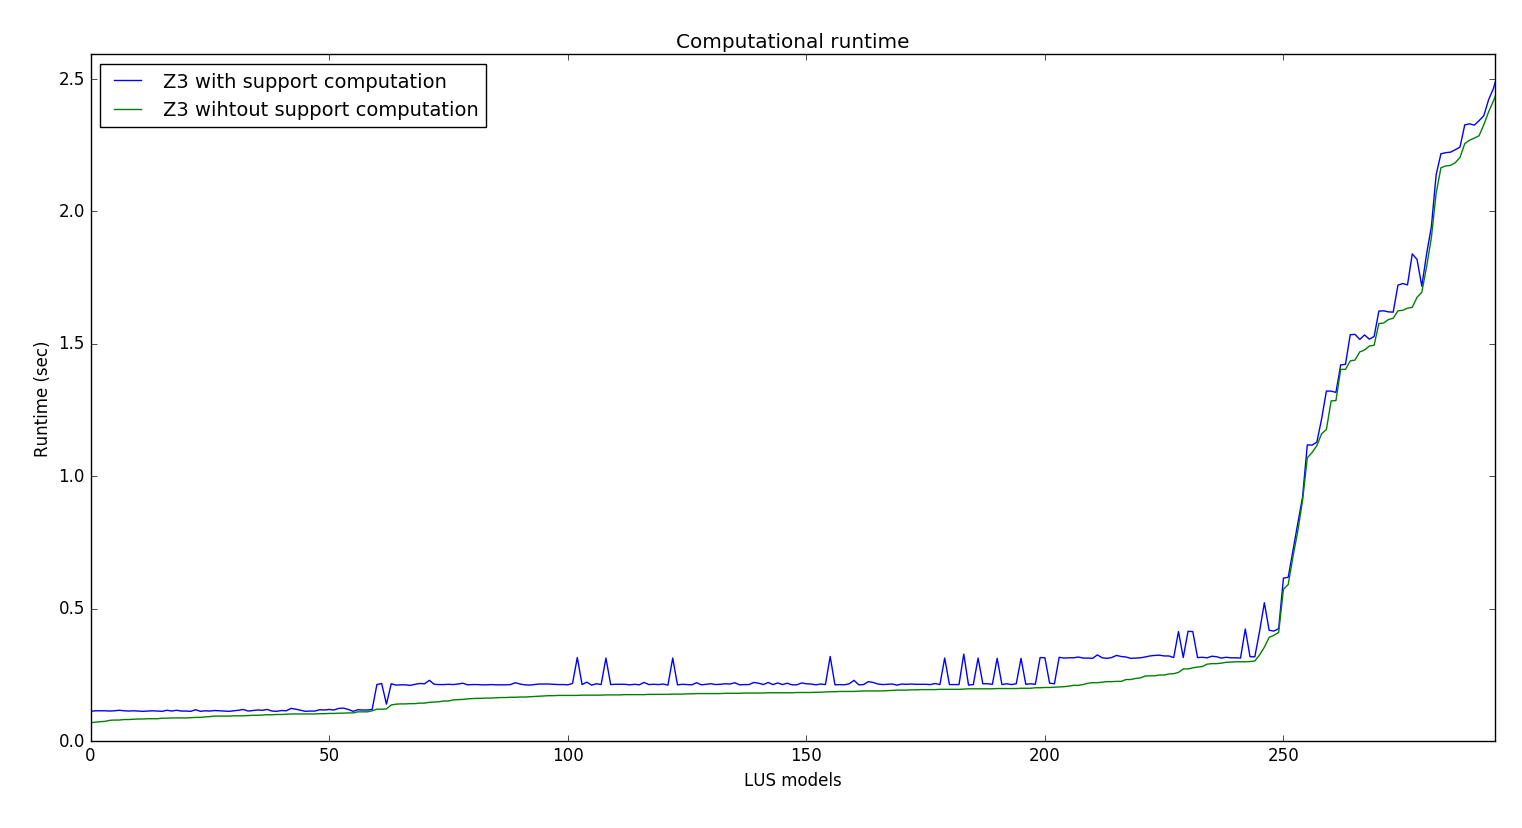
\includegraphics[width=\columnwidth]{figs/runtimeZ3.png}
  \caption{Runtime of \texttt{JKind} with/without support computation}\label{fig:runtimez3}
\end{figure}


\begin{figure}
  \centering
  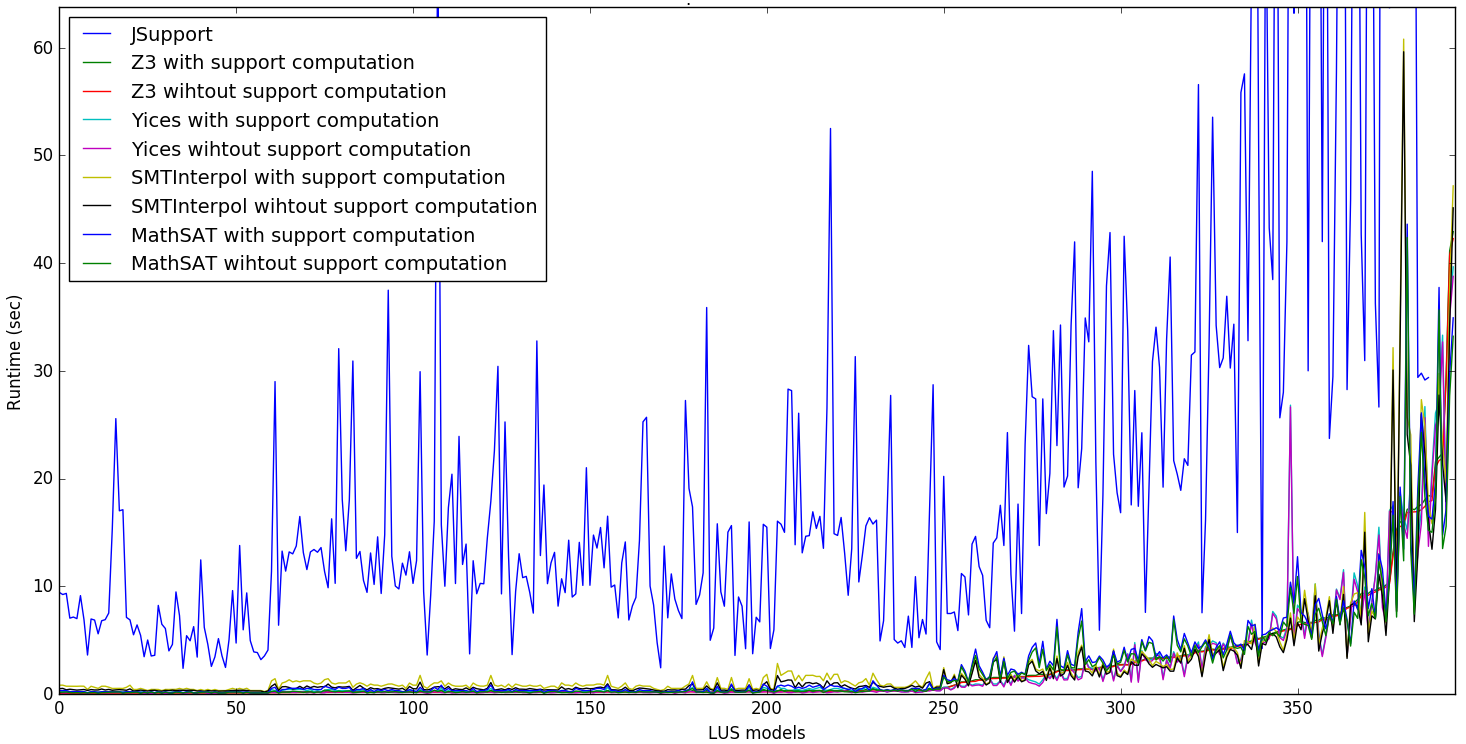
\includegraphics[width=\columnwidth]{figs/runtimeAll.png}
  \caption{Runtime of support computation with all solvers compared to \texttt{JSupport}}\label{fig:runtimeall}
\end{figure}
\noindent\fbox{%
    \parbox{\columnwidth}{%
        Support computation by \texttt{JSupport} is much more time-consuming than \texttt{ReduceSupport}.
    }%
}
 \vspace{6pt}

%\item \textbf{RQ2:} How close to minimal are the support sets computed by \texttt{ReduceSupport} vs. \texttt{JSupport}?
\textbf{RQ2.} To address this question, we begin by formulating the following statistical hypotheses:

\begin{itemize}
  \item H0: support sets computed by \texttt{ReduceSupport} are far away from minimal (i.e. an average Jaccard distance near 0.50, or an average size difference near 50\%).
  \item H1: support sets computed by \texttt{ReduceSupport} are close to minimal.
\end{itemize}

We calculated pairwise Jaccard distance between sets obtained from different configurations and \texttt{JSupport} per model. Then, minimum, maximum, mean, and standard deviation of the calculated data were obtained among all models.
The result are summarized as follows:
\begin{itemize}
  \item minimum of Jaccard distances from \texttt{JSupport} among all models is: 0.0
  \item maximum of Jaccard distances from \texttt{JSupport} among all models is: 0.882
  \item standard deviation for Jaccard distances from \texttt{JSupport} among all models is: 0.034
  \item average of Jaccard distances from \texttt{JSupport} is: 0.103
\end{itemize}
%\begin{table}
%  \centering
%  \begin{tabular}{ |c|c|c|c|c|c| }
%    \hline
%     min & max & mean & stdev & sample size& p-value\\[0.5ex]
%    \hline
%     0.0   & 0.882 & 0.103 & 0.034 & 4196 & < 0.00001 \\[0.5ex]
%    % mean H0 = 0.5
%    % sample_size = (405-10-8)*12 - (112*4) = 4644 - 448 = 4196  ---> sqrt = 64.78
%    % t-score =  mean - mean_H0 / (stdev / \sqrt{sample_zize}) = -756.40
%    \hline
%  \end{tabular}
%  \caption{Jaccard distances from \texttt{JSupport} among all models}
%  \label{tab:jsupjac}
%\end{table}

In terms of size, we calculated the size of the biggest and smallest sets per model, then added them together for all models. The same calculation has been done for \texttt{JSupport}:
\begin{itemize}
  \item $A\_JS$: the aggregate number of elements in support sets computed by \texttt{JSupport} = 3078
  \item $A\_Ss$: the aggregate number of elements in the \emph{smallest} support sets = 3474;
  this implies $A\_Ss$ is 12\% greater than $A\_JS$.
  \item $A\_Bs$: the aggregate number of elements in the \emph{biggest} support sets = 3586;
  this implies $A\_Bs$ is 16\% greater than $A\_JS$.
\end{itemize}
Average size of sets computed by \texttt{ReduceSupport} is 8.55. And, average size of sets computed by \texttt{JSupport} is 7.60. Therefore, in average, support sets computed by \texttt{ReduceSupport} are 88\% close to minimal, in terms of their size.  %  (1 - ((8.55 - 7.6)/ 7.6))  * 100 = 87.5%
Since \texttt{JSupport}, with a great percentage, most of the time computed the smallest support set, we compared the size of the sets computed by \texttt{ReduceSupport} with \texttt{JSupport}. For each configuration, we collected the difference between its support size and \texttt{JSupport} per model.
Then, minimum, maximum, average, and standard deviation of the collected data have been reported in Table~\ref{tab:minimality}. For example, -2 in the first column means that there was a case study where \texttt{ReduceSupport} generated sets that were smaller than the one computed by \texttt{JSupport} with a size difference of 2.

%
%
%\begin{figure}
%  \centering
%  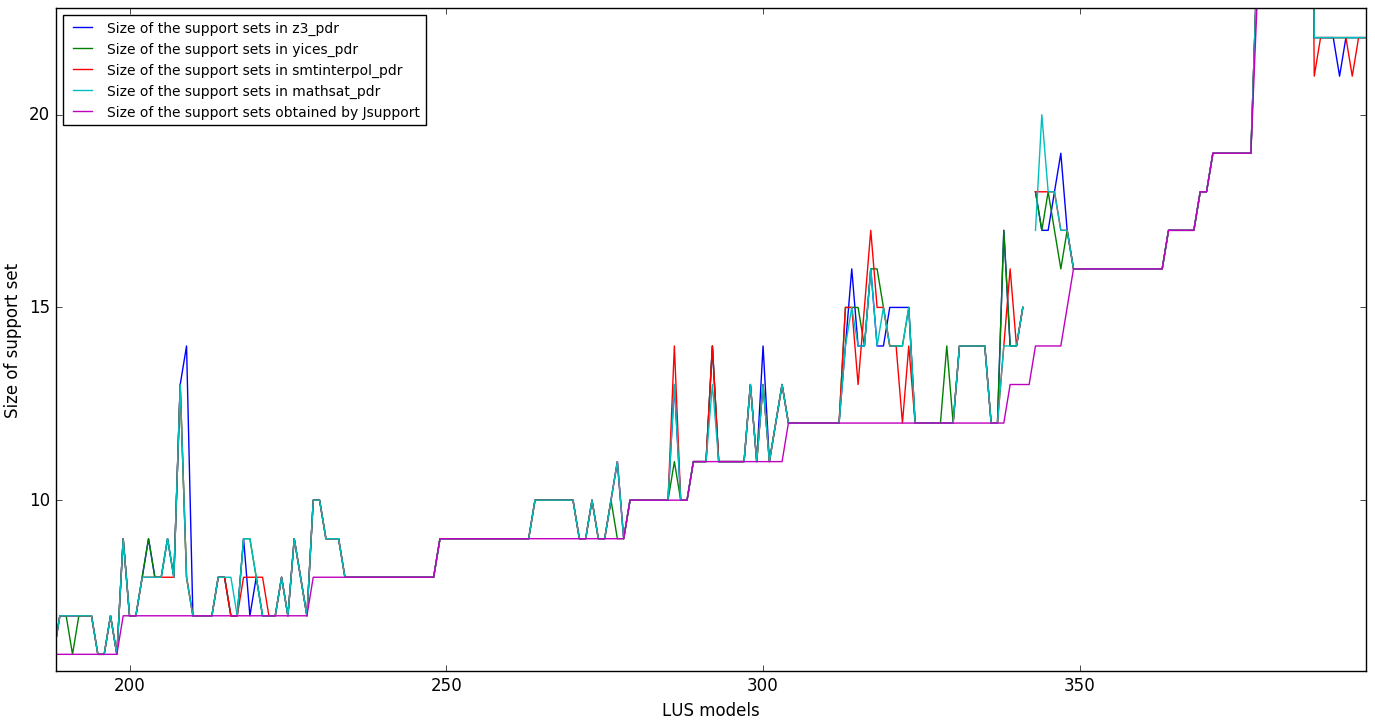
\includegraphics[width=\textwidth]{figs/minimality_pdr.png}
%  \caption{\small{Minimality comparison of \texttt{PDR}}}\label{fig:minpdr}
%\end{figure}
%
%
%\begin{figure}
%  \centering
%  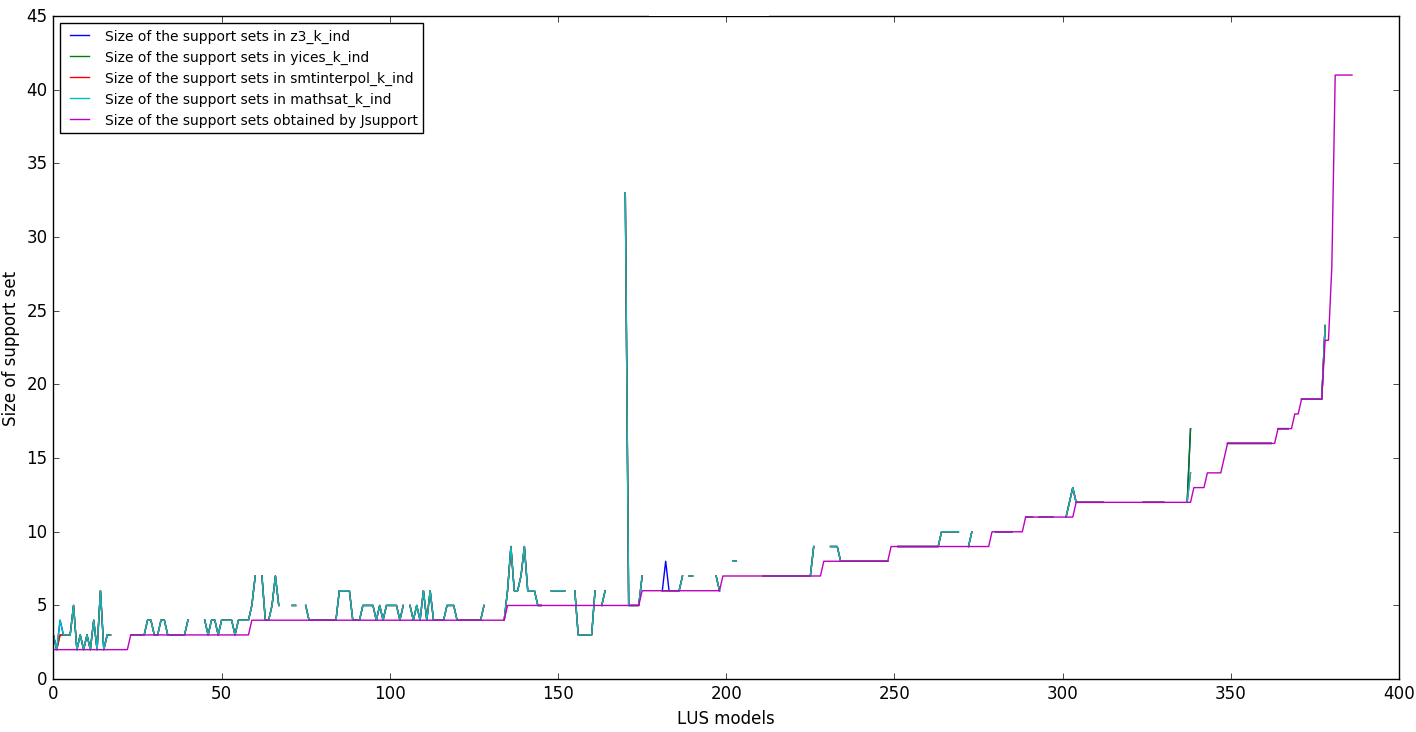
\includegraphics[width=\textwidth]{figs/minimality_kind.png}
%  \caption{\small{Minimality comparison of \texttt{K-induction}}}\label{fig:minkind}
%\end{figure}
%
%
%\begin{figure}
%  \centering
%  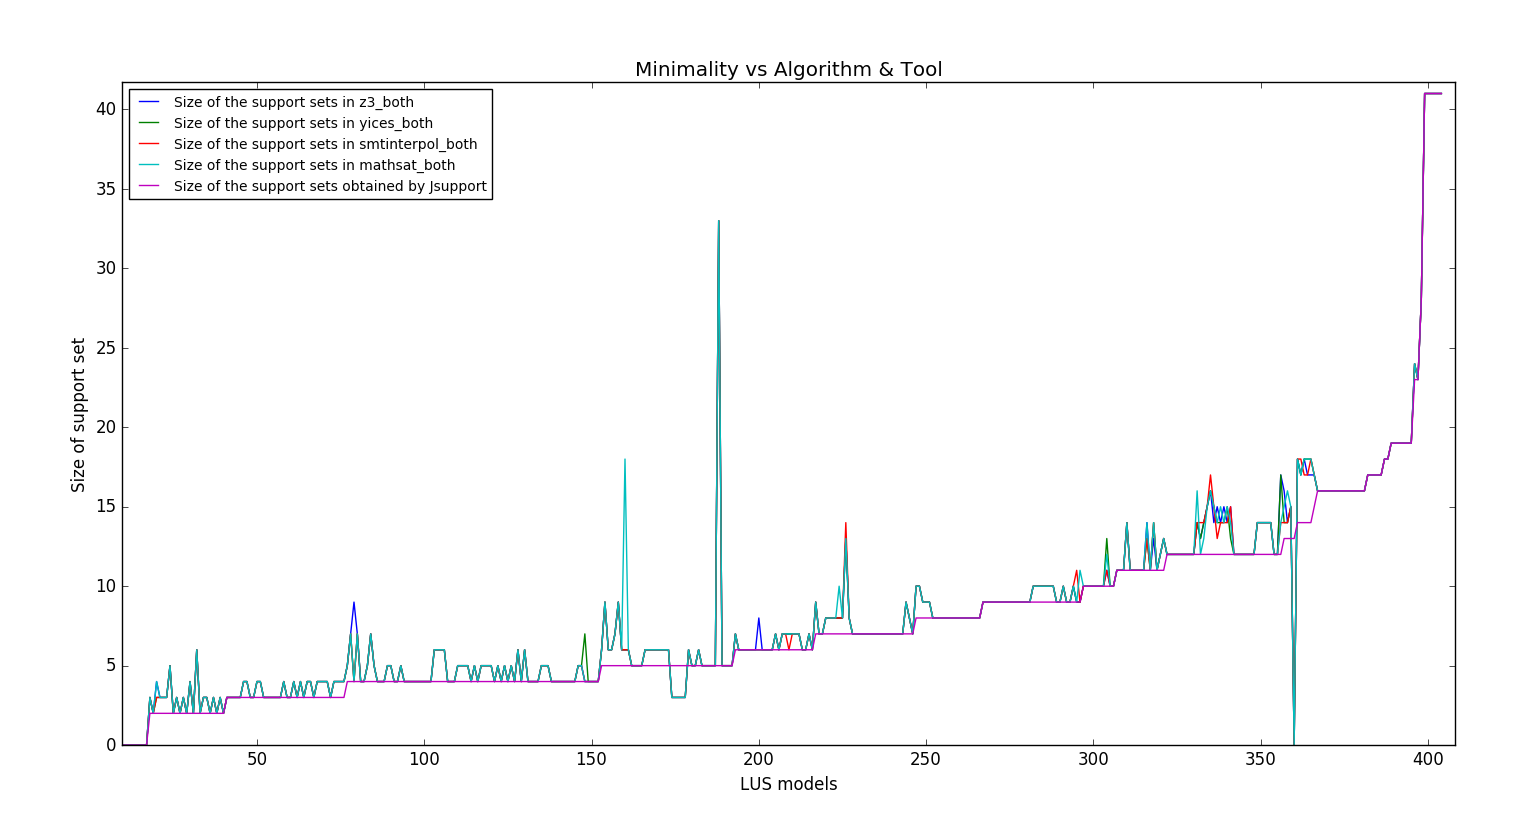
\includegraphics[width=\textwidth]{figs/minimality_both.png}
%  \caption{\small{Minimality comparison of \texttt{K-induction} and \texttt{PDR} working together}}\label{fig:minboth}
%\end{figure}
%
%
\begin{table}
  \centering
  \begin{tabular}{|c|c|c|c|c|}
     \hline
     configuration & min & max & mean & stdev \\[0.5ex]
     \hline\hline
     K-induction & -2 & 28 & 0.542 & 1.831 \\[0.5ex]
     PDR & -2 & 28 & 0.677 & 1.819 \\[0.5ex]
     Both engines & -2 & 28 & 0.661 & 1.751 \\[0.5ex]
     \hline
     Z3, K-ind & -2 & 28 & 0.555 & 1.842 \\[0.5ex]
     Yices, K-ind & -2 & 28 & 0.544 & 1.838 \\[0.5ex]
     SMTInterpol, K-ind & -2 & 28 & 0.534 & 1.822 \\[0.5ex]
     MathSAT, K-ind & -2 & 28 & 0.537 & 1.823 \\[0.5ex]
     \hline
     Z3, PDR & -2 & 28 & 0.697 & 1.852 \\[0.5ex]
     Yices, PDR & -2 & 28 & 0.668 & 1.807 \\[0.5ex]
     SMTInterpol, PDR & -2 & 28 & 0.673 & 1.813 \\[0.5ex]
     MathSAT, PDR & -2 & 28 & 0.668 & 1.803 \\[0.5ex]
     \hline
     Z3, Both engines & -2 & 28 & 0.663 & 1.729 \\[0.5ex]
     Yices, Both engines & -2 & 28 & 0.650 & 1.721 \\[0.5ex]
     SMTInterpol, Both engines & -2 & 28 & 0.637 & 1.713 \\[0.5ex]
     MathSAT, Both engines & -2 & 28 & 0.692 & 1.837 \\[0.5ex]
     \hline
   \end{tabular}
  \caption{Summary of minimality analyses in different configurations}\label{tab:minimality}
\end{table}

%\begin{figure}
%  \centering
%  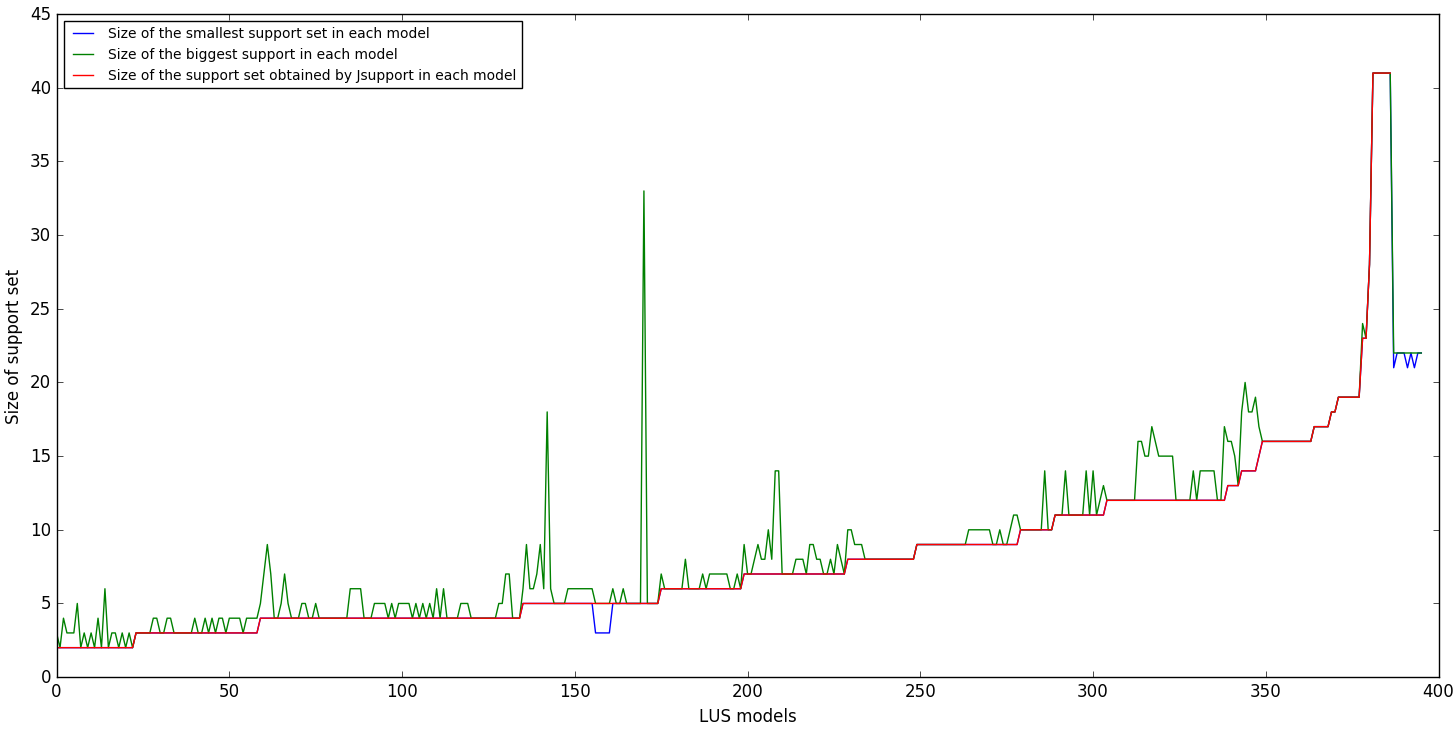
\includegraphics[width=\textwidth]{figs/minimality_analyses.png}
%  \caption{\small{Minimality comparison}}\label{fig:minjsup}
%\end{figure}


%
%\vspace{6pt}
%\noindent\fbox{%
%    \parbox{\textwidth}{%
%     \texttt{JKind} is able to find minimal support sets with a very negligible dependency on solvers/ proof engines.
%    }%
%}
% \vspace{6pt}
%
\vspace{6pt}
\noindent\fbox{%
    \parbox{\columnwidth}{%
     \texttt{ReduceSupport} computes set of supports that are very close to minimal, in terms of both size and similarity, with a very negligible dependency on solvers/ proof engines.
    }%
}
 \vspace{6pt}

%RQ3:  Does one solver/proof engine outperform others in terms of performance or minimality?
\textbf{RQ3.}   For this question, we consider performance and minimality separately.  We also analyzed the results from different aspects. The following describes methods used for analyzing and their results.

\textbf{(1)} For 405 models, we calculated minimum, maximum, avgerage, and standard deviation of Jaccard distance between \texttt{JSupport} and each configuration. To see if our computation is dependent on a particular solver/ proof engine, we formulate these hypotheses:
\begin{itemize}
  \item H0: \texttt{ReduceSupport} in some configurations generates support sets that are always far from minimal (with an average Jaccard distance near 0.5)
  \item H1: \texttt{ReduceSupport} in all configurations computes sets that are very close to minimal.
\end{itemize}

Table~\ref{tab:jsupconf} represents the result of this analysis; for example, configuration \emph{(Z3, Both)}, shows that \texttt{JKind} with \texttt{Z3} and both \texttt{K-induction} and \texttt{PDR} engines has an average Jaccard distance of 0.106 (in 405 models) from \texttt{JSupport}.


\begin{table}
  \centering
  \begin{tabular}{|c|c|c|c|c|}
    \hline
    configuration & min & max & mean & stdev  \\[0.5ex]
    \hline\hline
    % sample size = 405 - 18 = 387    sample size for k_ind = 405 - 18 - 112 = 275
    %
    Z3, Both & 0.0 & 0.882 & 0.106 & 0.155 \\[0.5ex]
    Z3, K-induction & 0.0 & 0.882 & 0.116 & 0.168 \\[0.5ex]
    z3, PDR & 0.0 & 0.882 & 0.102 & 0.151 \\[0.5ex]
    \hline
    Yices, Both & 0.0 & 0.882 & 0.104 & 0.152 \\[0.5ex]
    Yices, K-induction & 0.0 & 0.882 & 0.114 & 0.166 \\[0.5ex]
    Yices, PDR & 0.0 & 0.882 & 0.098 & 0.147 \\[0.5ex]
    \hline
    SMTInterpol, Both & 0.0 & 0.882 & 0.103 & 0.152 \\[0.5ex]
    SMTInterpol, K-induction & 0.0 & 0.882 & 0.115 & 0.167 \\[0.5ex]
    SMTInterpol, PDR & 0.0 & 0.882 & 0.101 & 0.149 \\[0.5ex]
    \hline
    MathSAT, Both & 0.0 & 0.882 & 0.106 & 0.156 \\[0.5ex]
    MathSAT, K-induction & 0.0 & 0.882 & 0.115 & 0.167 \\[0.5ex]
    MathSAT, PDR & 0.0 & 0.882 & 0.100 & 0.148 \\[0.5ex]
    \hline
  \end{tabular}
  \caption{Jaccard distance between \texttt{JSupport} and each configuration}\label{tab:jsupconf}
\end{table}

\vspace{6pt}
\noindent\fbox{%
    \parbox{\columnwidth}{%
    \texttt{ReduceSupport}, regardless of solver/ proof engine, generated support sets that are very close to minimal sets computed by \texttt{JSupport}.
    }%
}
 \vspace{6pt}

% H0: there are pairwise configurations that generate support sets that are very different (with an average Jaccard distance near 0.5)
\textbf{(2)} For each model in the benchmark, the experiments generated 13 different sets of support.
We used Jaccard distance to measure dissimilarity between pairwise of these sets
Therefore, we obtained $\binom{13}{2} = 78$ combinations of distances per model. Then, minimum, maximum, average, and standard deviation of the distances were calculated (Fig~\ref{fig:jacdis}), by which, again, we calculated these four measures among all 405 models. The following summarizes the result of this analysis:
\begin{itemize}
  \item minimum Jaccard distance among all models is: 0.0
  \item maximum Jaccard distance among all models is: 0.882
  \item average Jaccard distance among all models is: 0.027
  \item standard deviation of Jaccard distance among all models is: 0.062
\end{itemize}

\begin{figure}
  \centering
  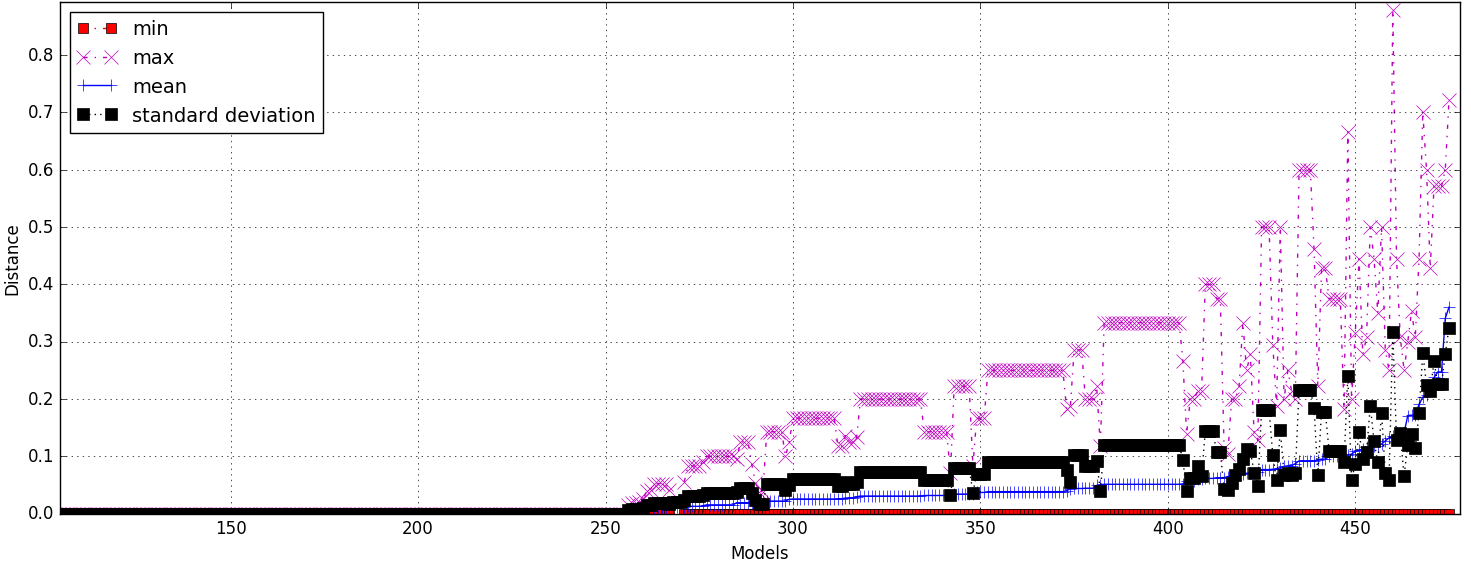
\includegraphics[width=\columnwidth]{figs/jacdis2.png}
  \caption{\small{Pairwise Jaccard distance between support sets}}\label{fig:jacdis}
\end{figure}


\vspace{6pt}
\noindent\fbox{%
    \parbox{\columnwidth}{%
        Support sets computed with different solvers and engines have an average Jaccard distance of 0.027, which implies our algorithm has very small dependency on tools and proof algorithms.
        In addition, it also implies the generated sets are very close to each other.
    }%
}
 \vspace{6pt}

%\textbf{(3)}  Fig~\ref{fig:maxdis} and Fig~\ref{fig:mindis} shows the results. As you can see, different configurations of \texttt{JKind} do not affect very much the variety of the generated sets. However, \texttt{JSupport} and \texttt{JKind} configurations have had maximum distances most of the time. Even so, the frequency of such maximum distances among 405 models is very low. Table~\ref{tab:pairminmax} shows the percentage that two configurations has the maximum Jaccard distance
%\ela{this is a misleading approach because maximum jaccard distance doesn't mean a big jaccard distance. for this reason, I remove it. related results for this section is in file support_variety_analyses.txt }

%\begin{figure}
%  \centering
%  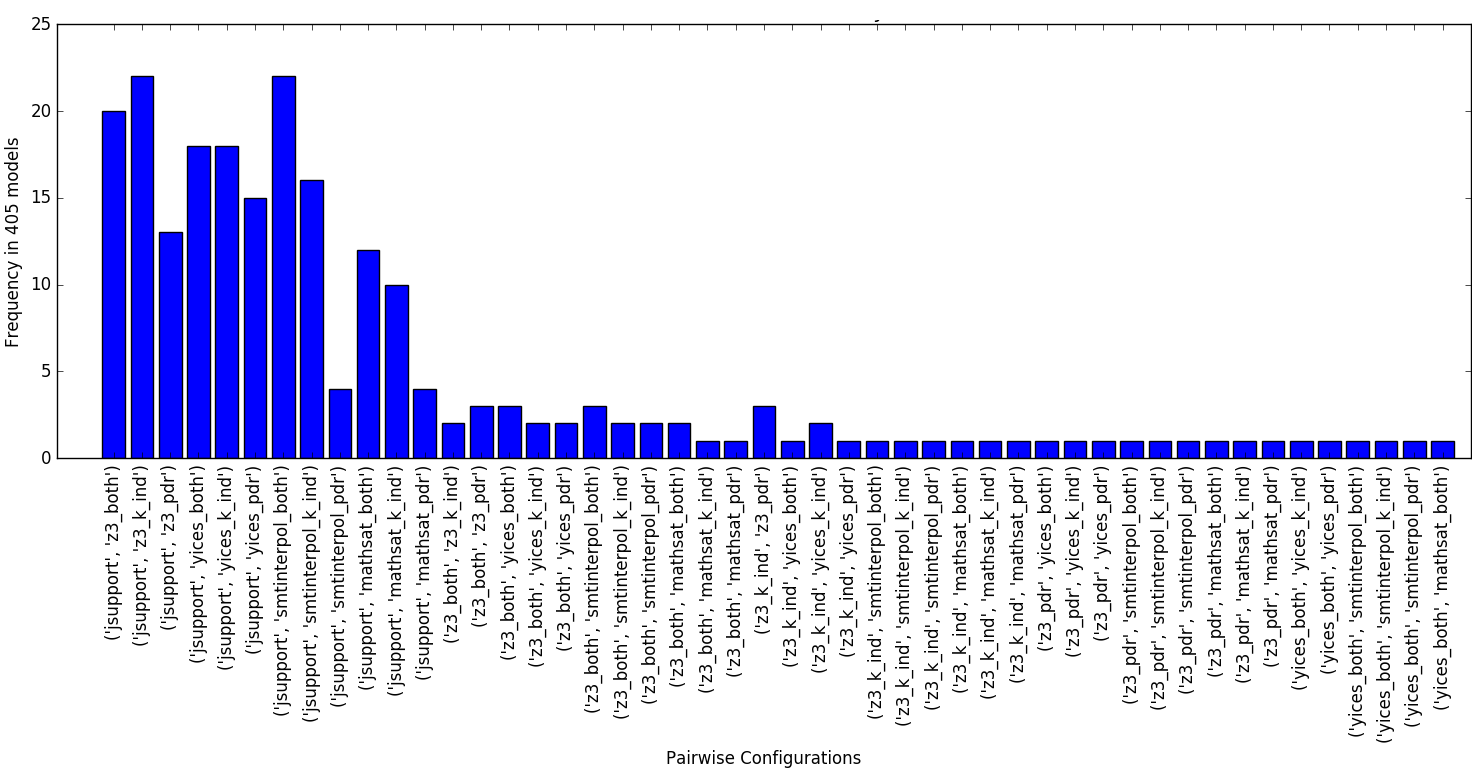
\includegraphics[width=\textwidth]{figs/max_settings_analyses.png}
%  \caption{\small{Pairwise configurations with maximum Jaccard distance}}\label{fig:maxdis}
%\end{figure}
%
%
%\begin{figure}
%  \centering
%  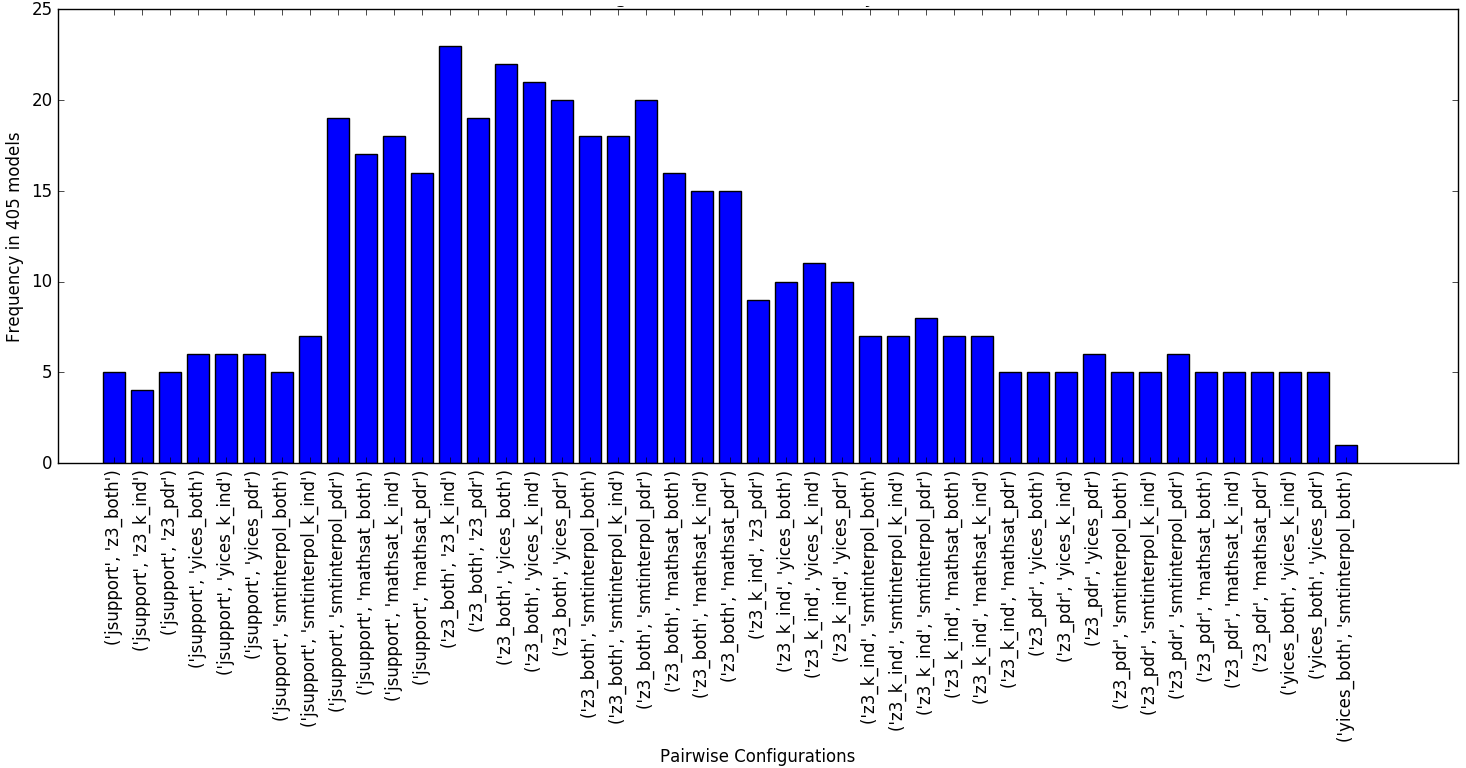
\includegraphics[width=\textwidth]{figs/min_settings_analyses.png}
%  \caption{\small{Pairwise configurations with minimum Jaccard distance}}\label{fig:mindis}
%\end{figure}

%\vspace{6pt}
%\noindent\fbox{%
%    \parbox{\textwidth}{%
%        Different solvers and proof engines have very small impact on the variety of elements in a support set of a property computed by our algorithm.
%    }%
%}
% \vspace{6pt}

\textbf{Timing analysis.} Table~\ref{tab:eff-comp-jsup} compares overall runtime of support computation in different solvers and \texttt{JSupport}, which helps to see if any solvers outperform others in terms of performance.

\begin{table}
  \centering
  \begin{tabular}{ |c||c|c|c|c| }
    \hline
     runtime (sec) & min & max & mean & stdev \\[0.5ex]
    \hline\hline
    JSupport & 2.381 & 165.157 & 21.533 & 23.533 \\[0.5ex]
    Z3   & 0.112 & 42.928 & 2.412 & 5.009 \\[0.5ex]
    Yices &   0.111  & 39.657   & 2.464 & 5.224 \\[0.5ex]
    SMTInterpol& 0.225 & 514.886 &  4.331 & 26.411 \\[0.5ex]
    MathSAT & 0.111 & 43.623 &  2.765 & 5.157 \\[0.5ex]
    \hline
  \end{tabular}
  \caption{\small{\texttt{ReduceSupport} runtime with different solvers compared to \texttt{JSupport}}}
  \label{tab:eff-comp-jsup}
\end{table}

%For calculations, we considered all settings where both \texttt{K-induction} and \texttt{PDR} were activated
% then in for all 405 models in everything, we collected runtime info, then calculated min/max/avg/stdev between them
% in other words, there were 4 settings to be considered: z3_both, yices_both, mathsat_both, smtinterpol_both


%\begin{figure}
%\centering
%\begin{tabular}[c]{cc}
%    \begin{subfigure}[b]{0.20\textwidth}
%      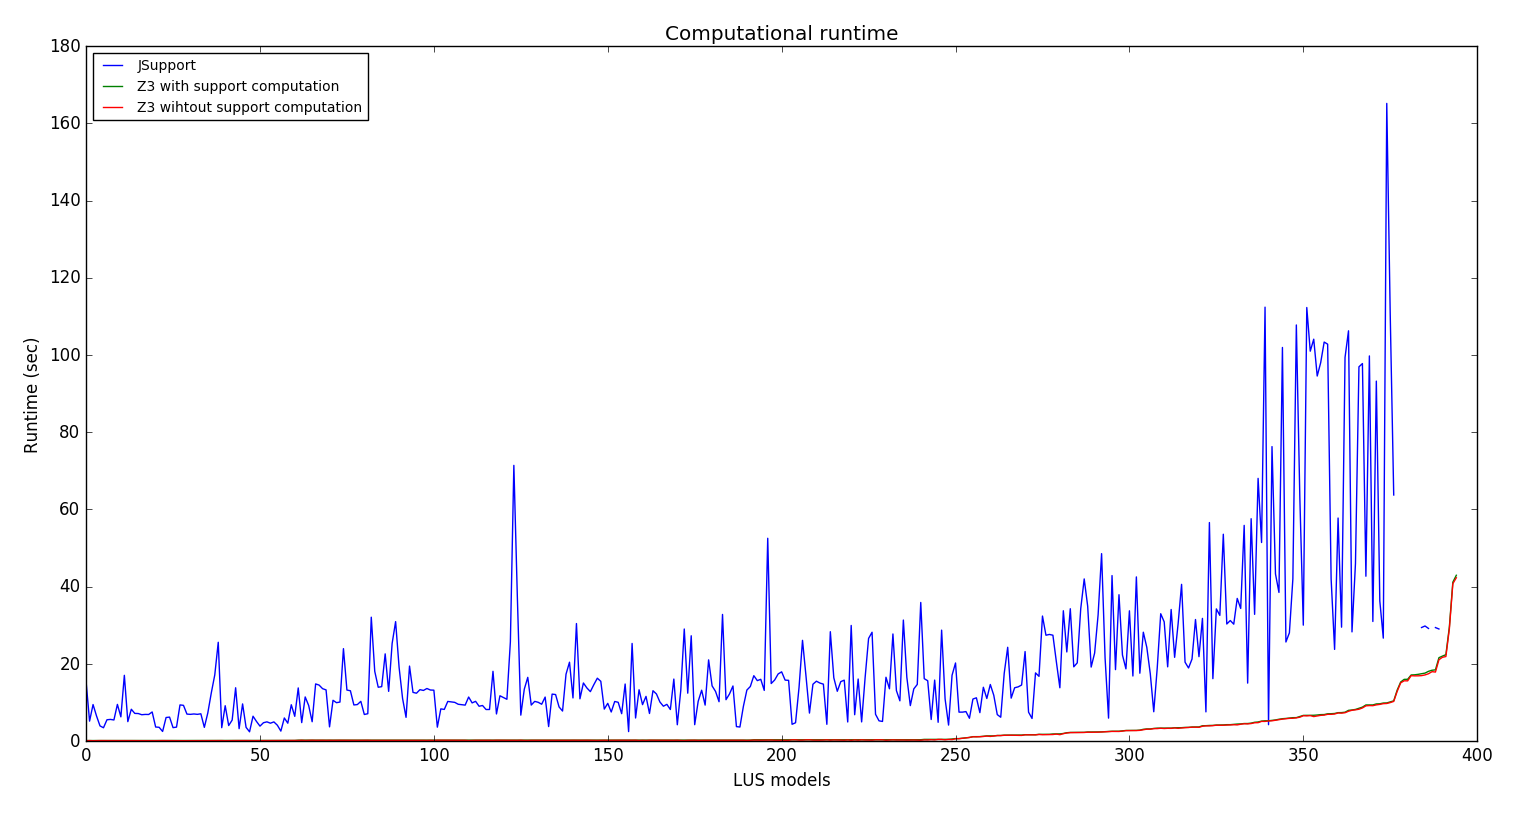
\includegraphics[width=\textwidth]{figs/figure_1.png}
%    \end{subfigure}&
%    \begin{subfigure}[b]{0.20\textwidth}
%      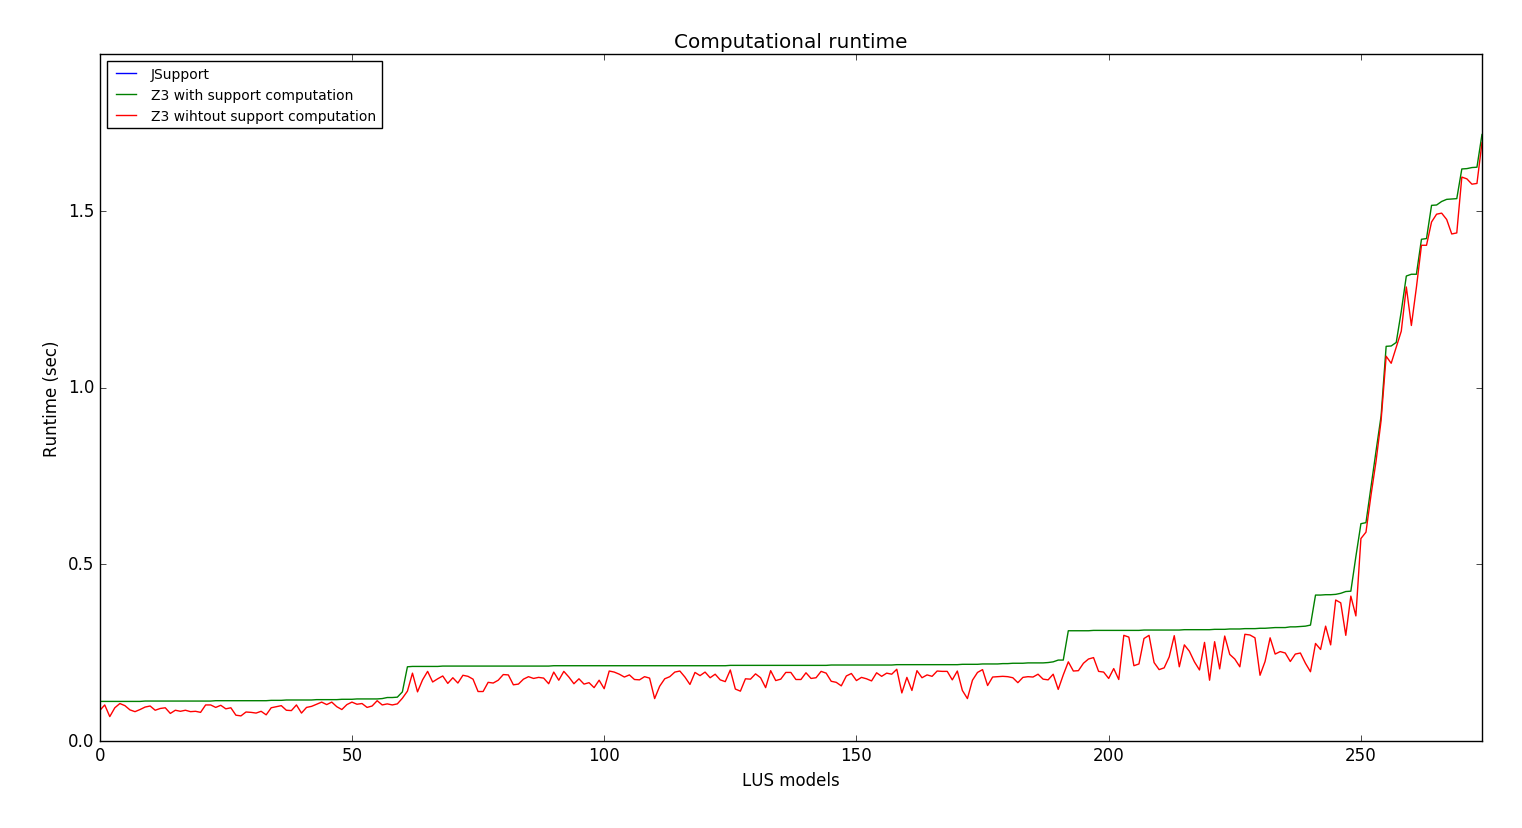
\includegraphics[width=\textwidth]{figs/figure_z3_zoom.png}
%    \end{subfigure}\\
%    \begin{subfigure}[b]{0.20\textwidth}
%      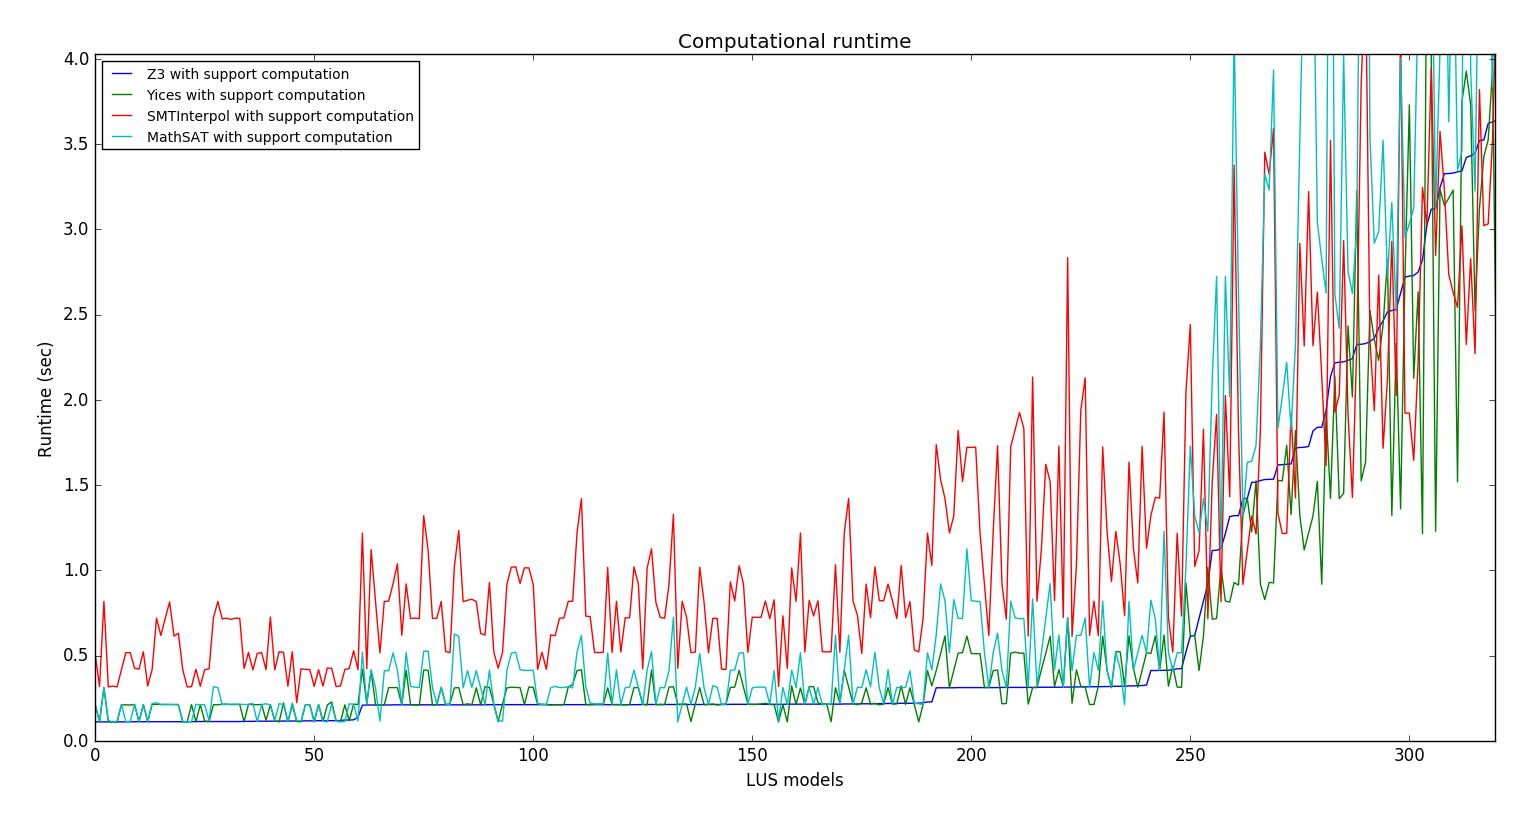
\includegraphics[width=\textwidth]{figs/solvers-support-zoom2.png}
%    \end{subfigure}&
%    \begin{subfigure}[b]{0.20\textwidth}
%      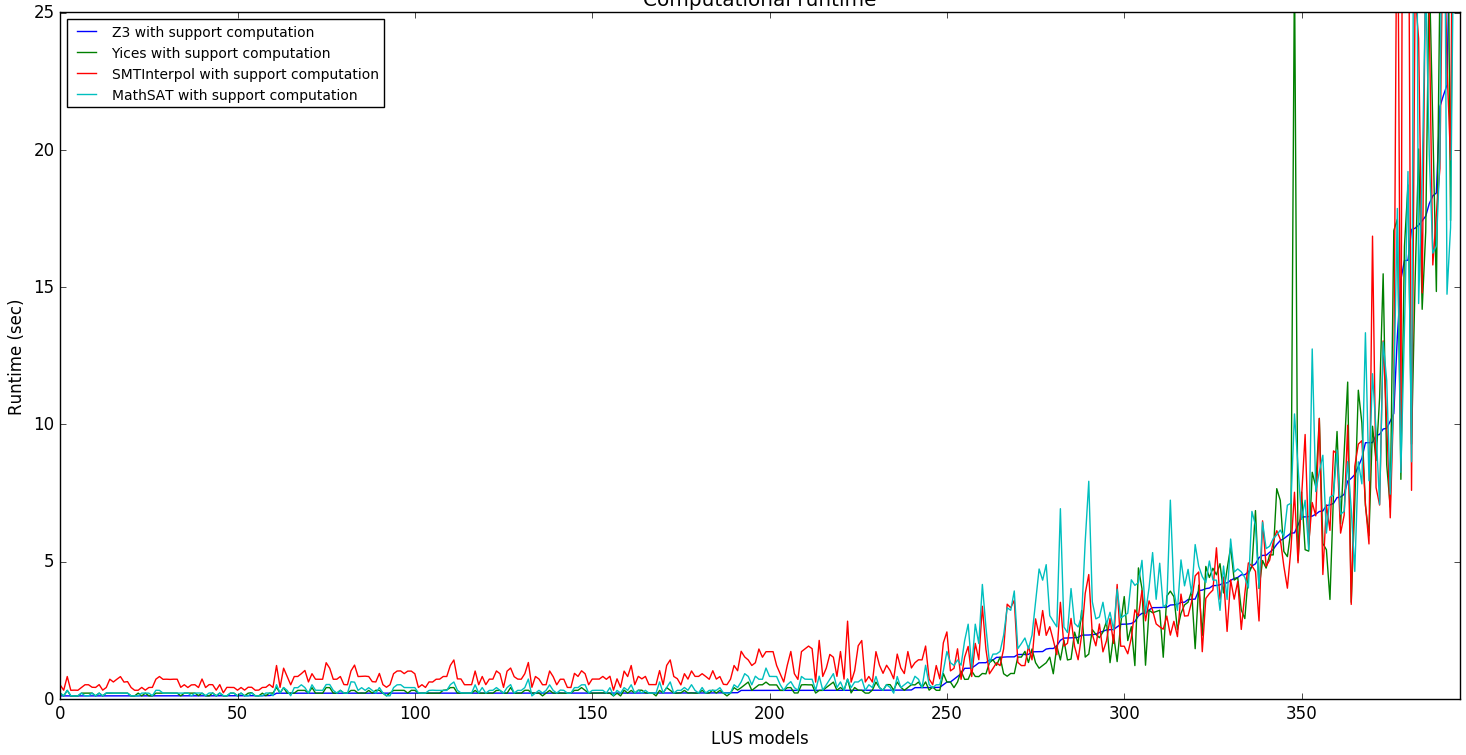
\includegraphics[width=\textwidth]{figs/solvers-support-zoom1.png}
%    \end{subfigure}
%  \end{tabular}
%\caption{\small{Runtime of support computation}}
%\label{fig:runtime}
%\end{figure}

\vspace{6pt}
\noindent\fbox{%
    \parbox{\columnwidth}{%
        Time-efficiency of \texttt{ReduceSupport} is not quite solver-dependent. However, SMTInterpol works less efficiently in comparison with others.
    }%
}
\vspace{6pt}
%
%
%
%% RQ3: Is there any relationship between the size of a computed support set and
%%solvers/ proof engines?
%\textbf{RQ3:} To address this question, we analyzed the raw data with two different approaches described in the following.
%
%\textbf{(1)} We analyzed the sets of each 405 models. In each model, we looked for configurations that generated the biggest support set and ones that generated the smallest. Fig~\ref{fig:smallest} and Fig~\ref{fig:bigest} visualize the results of this analysis. For example, as you can see in Fig~\ref{fig:bigest}, \texttt{JSupport} generated biggest support sets in less than 10 models. Note that it implies there is at least one \texttt{JKind} configuration that generated the set with a smaller size.
%
%
%\begin{figure}
%  \centering
%  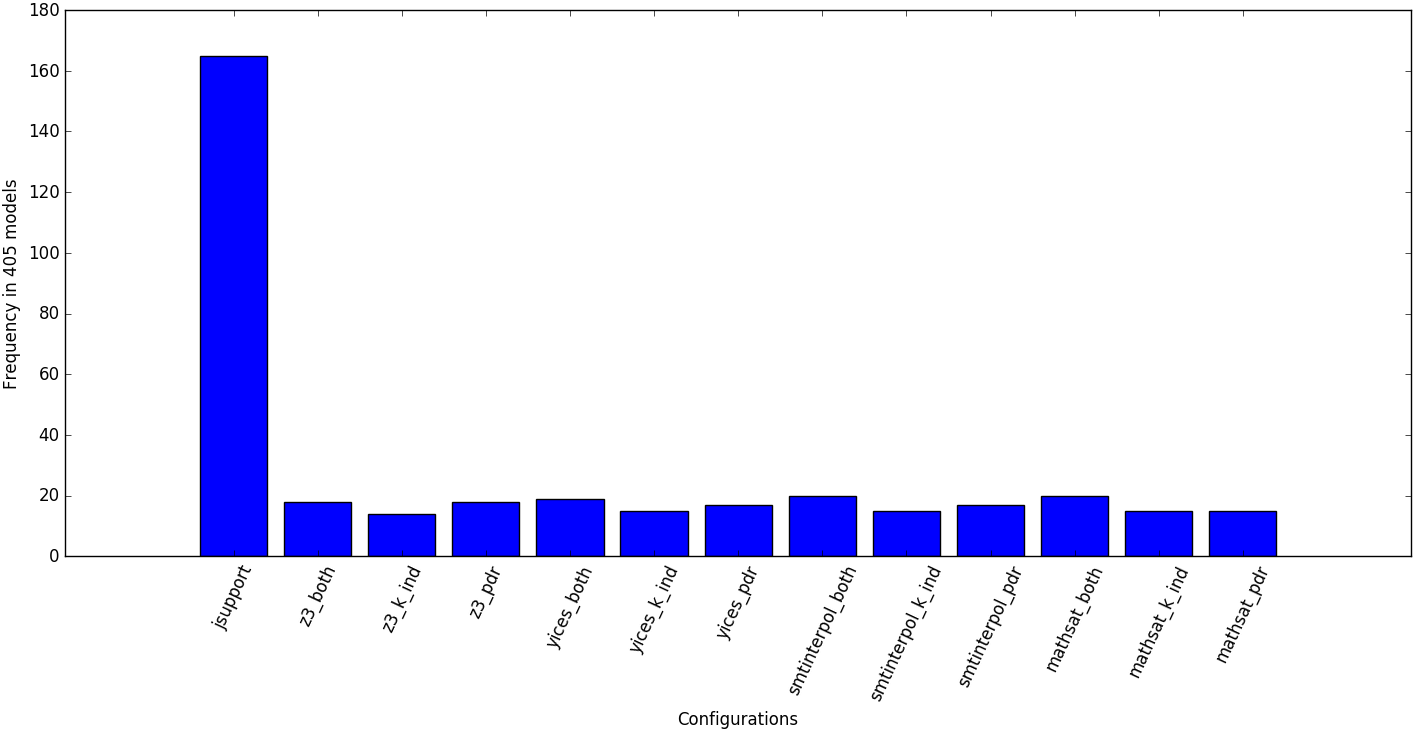
\includegraphics[width=\textwidth]{figs/small_conf.png}
%  \caption{\small{Smallest support set (in terms of size) vs configurations}}\label{fig:smallest}
%\end{figure}
%
%
%\begin{figure}
%  \centering
%  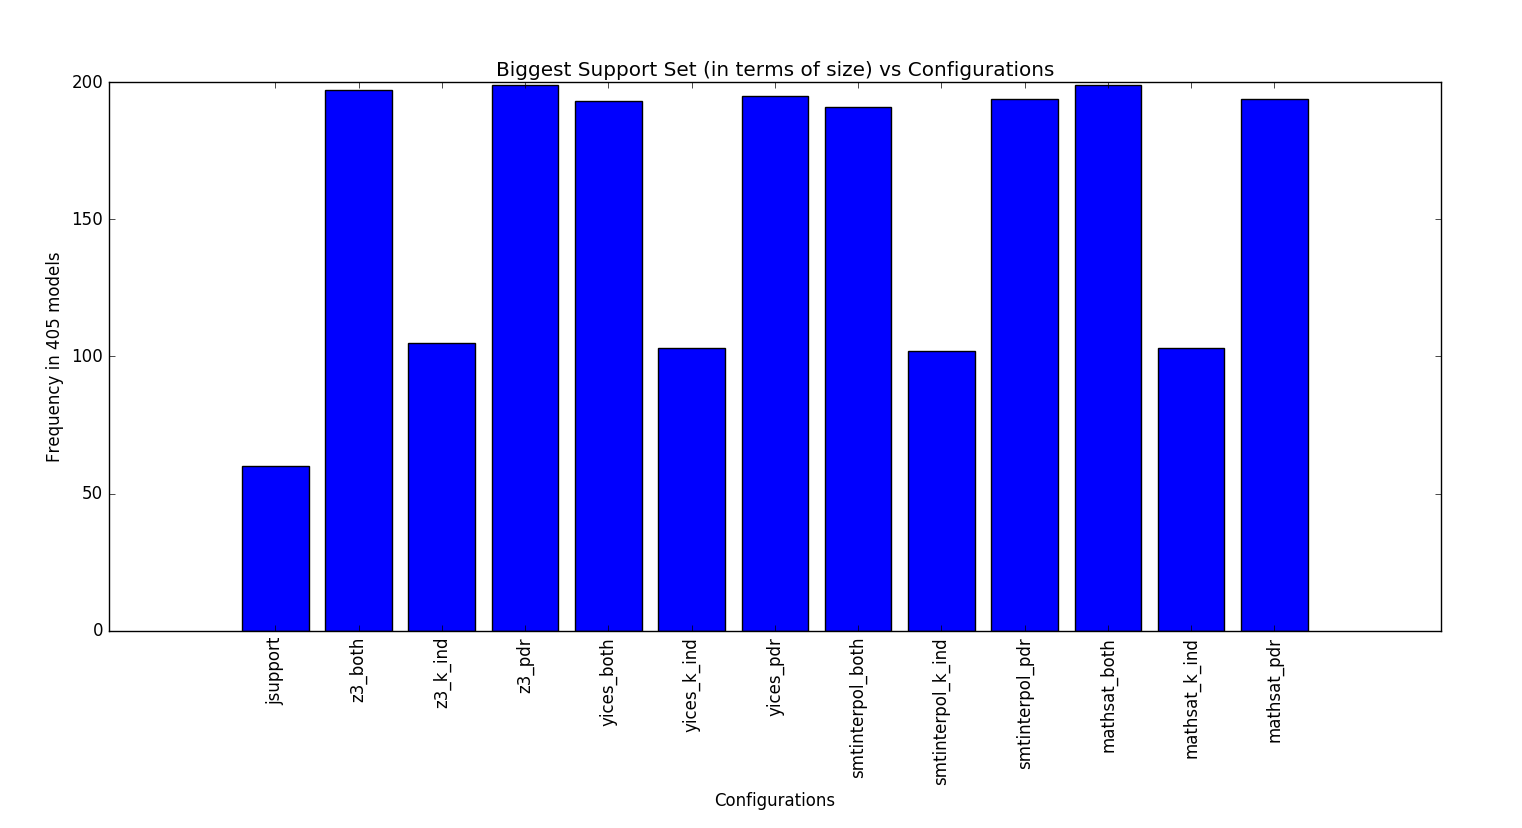
\includegraphics[width=\textwidth]{figs/big_conf.png}
%  \caption{\small{Biggest support set (in terms of size) vs configurations}}\label{fig:bigest}
%\end{figure}
%
%\vspace{6pt}
%\noindent\fbox{%
%    \parbox{\textwidth}{%
%    Solvers/ proof engines have negligible effects on the size of the support sets computed by \texttt{JKind}.
%    }%
%}
% \vspace{6pt}
%

%\textbf{RQ4:} How much {\em diversity} exists in the solutions produced by different configurations?
\textbf{RQ4.} To measure the overall similarity among all sets, instead of a pairwise comparison, we used \emph{frequent pattern mining} \cite{han2007frequent}. To define an overall similarity among all sets of support of a given model
\footnote{Note that all models in the benchmarks are single property; hence, instead of saying a set of support of a given \emph{property}, we just refer it as the support set of the \emph{model} while explaining the experimental results.}
, we calculated a \emph{core} support set for each model in the benchmark, which can be considered as a closed frequent pattern; a core set of model $M$, denoted by $C_M$, is defined as:
\begin{definition}
  \label{def:core}
  $C_M = \bigcap_{i=1}^{13} s_{Mi},   \hspace{9pt} s_{Mi} \in S_M$
\end{definition}

Based on this notion, overall dissimilarity, denoted by $D_{J\{M\}}$, is defined as follows:

\begin{definition}
  \label{def:dis}
  $D_{J\{M\}} =  \frac{\sum_{i=1}^{12}d_J(s_{Mi}, C_M)}{12},   \hspace{9pt} s_{Mi} \in S_M$
\end{definition}

Since our goal is to measure the diversity or dissimilarity among sets computed by \texttt{ReduceSupport}, in \ref{def:dis}, we exclude the set generated by \texttt{JSupport}. In Fig~\ref{fig:jacdis}, the \emph{overall distance} line shows $D_{J\{M\}}$ per model, which can be summarized as follows:
\begin{itemize}
  \item minimum $D_{J\{M\}}$ among all models: 0.0
  \item maximum $D_{J\{M\}}$ among all models: 0.879
  \item average $D_{J\{M\}}$ among all models: 0.096
  \item standard deviation of $D_{J\{M\}}$ among all models: 0.132
\end{itemize}

\vspace{6pt}
\noindent\fbox{%
    \parbox{\columnwidth}{%
    An average $D_{J\{M\}}$ of 0.096 shows that variety of support sets computed by \texttt{ReduceSupport} is very small.
    }%
}
 \vspace{6pt}

%\textbf{(3)} In addition to Jaccard distance, we also measured similarity among all sets computed in different configurations per model. Let $S_M$ be a set of all support sets computed for model $M$ (i.e. in our experiments, $S_M$ is a set of 13 sets).  We define similarity per model as follows:
%
%\begin{center}
%$similarity = \frac{|\bigcap_{i=1}^{13} s_{Mi}|}{|\bigcup_{i=1}^{13} s_{Mi}|}, \hspace{9pt} s_{Mi} \in S_M$
%\end{center}
%\vspace{6pt} \ela{should see if this formula has any name in mathematics?!}
%
%Needless to say, $0 \leq similarity \leq 1$, and if all the sets in $S_M$ are the same, \textit{similarity}will be 1. So the closer to 1 it is, the more similar sets $S_M$ has. Fig~\ref{fig:sim} shows similarity in all models. Here is also a summary of minimum, maximum, average, and standard deviation of similarity among all models:
%\begin{itemize}
%  \item minimum similarity among all models is: 0.12
%  \item maximum similarity among all models is: 1.0
%  \item average similarity among all models is: 0.884
%  \item standard deviation of similarity among all models is: 0.165
%\end{itemize}
%
%
%\begin{figure}
%  \centering
%  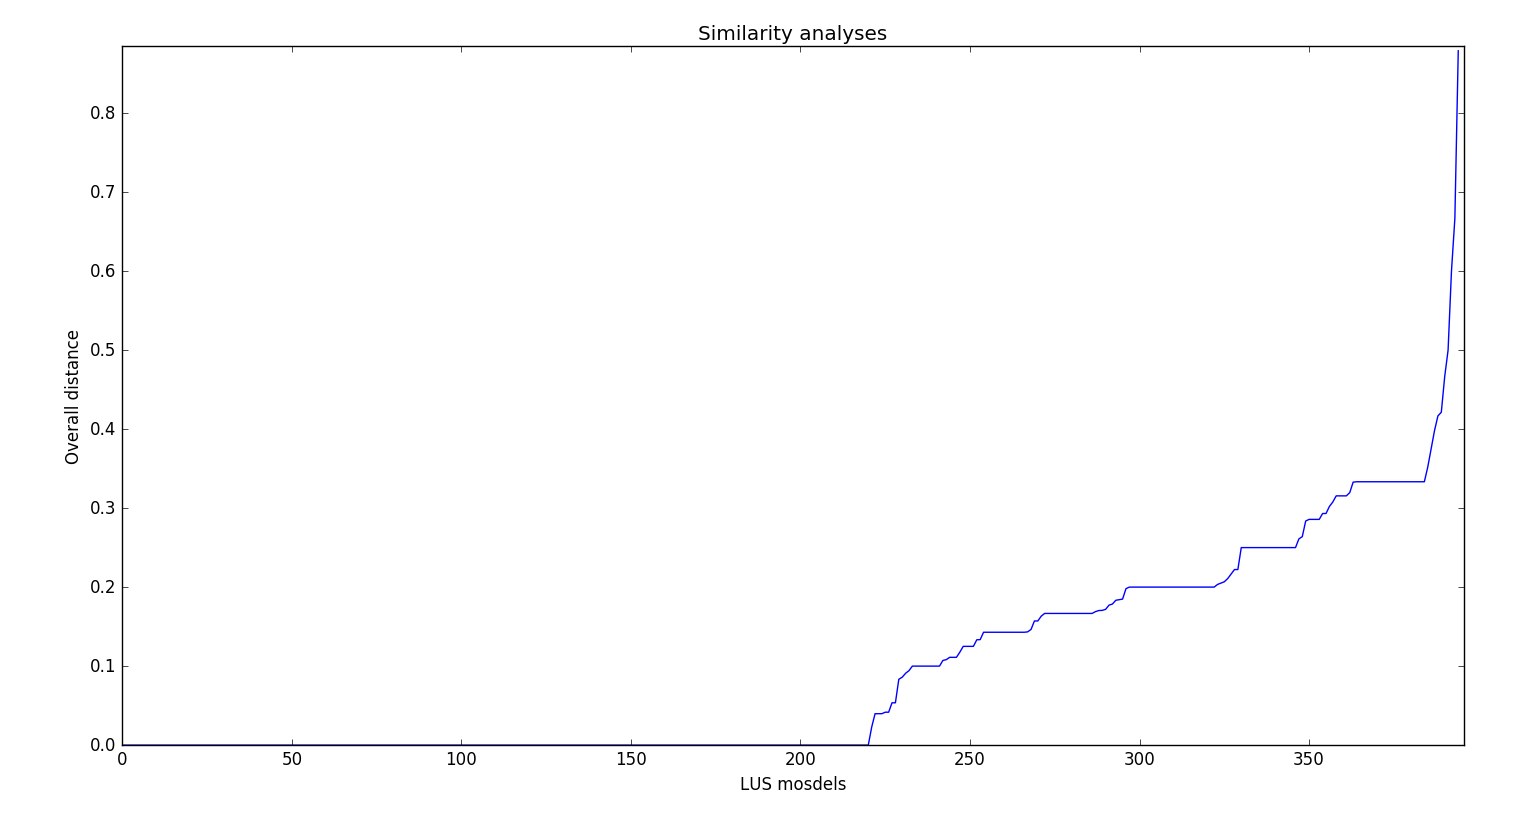
\includegraphics[width=\textwidth]{figs/similarity.png}
%  \caption{\small{Similarity measurement for all models}}\label{fig:sim}
%\end{figure}
%
%\vspace{6pt}
%\noindent\fbox{%
%    \parbox{\textwidth}{%
%        An average \textit{similarity} of 0.884 shows that support sets computed in different
%        configurations are very similar. So, the dependency of our algorithm to different solvers and proof engines is negligible.
%    }%
%}
% \vspace{6pt}
%
%\textbf{(4)}  The results are visualized in Fig~\ref{fig:core}.
%
%
%\begin{figure}
%  \centering
%  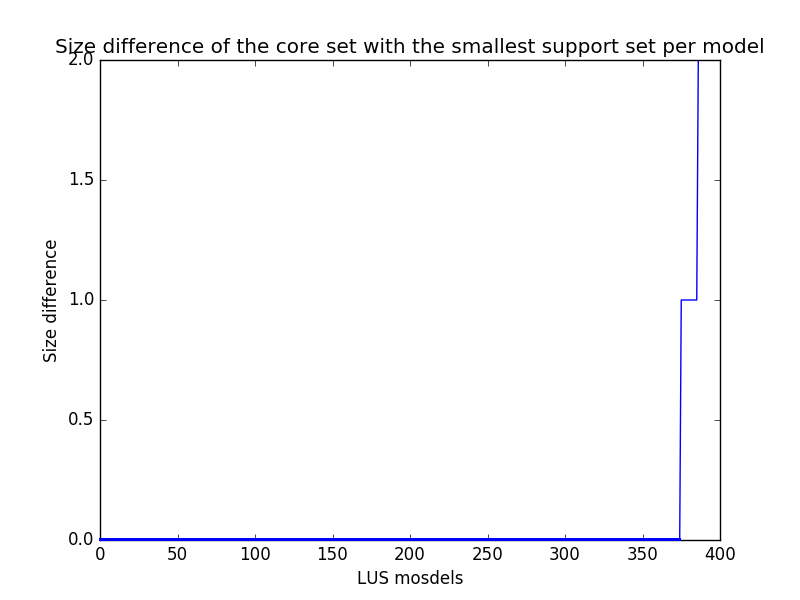
\includegraphics[width=\textwidth]{figs/core.png}
%  \caption{\small{Size difference between the core set and the smallest support set per model}}\label{fig:core}
%\end{figure}
%
%\vspace{6pt}
%\noindent\fbox{%
%    \parbox{\textwidth}{%
%        The core support set is very close to the smallest support set of a property.
%    }%
%}
% \vspace{6pt}



%\item \textbf{RQ5:} How does model size affect minimality and diversity of solutions?
\textbf{RQ5.} The size of the models in our benchmark is between 0 KB and 10 KB.
We divided the models into 9 different categories based on their size such that $category_i$ contains
all models whose sizes are between $(i - 1)$ KB and $i$ KB. Then, using Definition~\ref{def:dis}, distance for each model in each category was calculated. After that, minimum, maximum, average, standard deviation of the data were obtained per category. Table~\ref{tab:modelsize} summarizes the result of this analysis; the column \emph{number} in the table shows the number of models in each category, which means the sum of the numbers in the column is 405 (for example, there are 6 models whose sizes are between 8 KB and 9 KB, and in all of them \textit{similarity} is 1.0).


\begin{table}
  \centering
  \begin{tabular}{ |c||c|c|c|c|c|}
    \hline
    size (KB) & number&
     min & max & mean & stdev \\[0.5ex]
    \hline\hline
    [0-1] & 49 & 0.0 & 0.333 & 0.084 & 0.131 \\[0.5ex]
    [1-2] & 90& 0.0 & 0.667 & 0.139 & 0.157 \\[0.5ex]
    [2-3] & 26&0.0 & 0.5 & 0.124 & 0.132 \\[0.5ex]
    [3-4] & 34&0.0 & 0.333 & 0.076 & 0.124 \\[0.5ex]
    [4-5] & 88&0.0 & 0.879 & 0.090 & 0.134 \\[0.5ex]
    [5-6] & 11&0.0 & 0.25 & 0.170 & 0.107 \\[0.5ex]
    [6-7] & 2&0.0 & 0.042 & 0.021 & 0.021 \\[0.5ex]
    [7-8] & 99&0.0 & 0.398 & 0.067 & 0.094 \\[0.5ex]
    [8-9] & 6&0.0 & 0.0 & 0.0 & 0.0 \\[0.5ex]
    \hline
  \end{tabular}
  \caption{Model size vs similarity among its support sets}\label{tab:modelsize}
\end{table}

\vspace{6pt}
\noindent\fbox{%
    \parbox{\columnwidth}{%
     The size of the model does not affect the stability of our algorithm;
     if a model is large, it does not mean that it will have a lot of different minimal support sets. In other words, minimal support sets of a given property computed by \texttt{JKind} will be very similar to each other.
    }%
}
 \vspace{6pt}

